\subsection{Xception}\label{resultsXceptions}

The implementation of the Xception architecture presented us with particular challenges right from the start, mainly because Xception is not included in the PyTorch model library. We resorted to the ``pretrainedmodels'' library to gain access to a pre-trained Xception model, although this is outdated (last update 2018). While the library's pretrained Xception model was operational, its use led to some further complications.
One major hurdle was adjusting the input size to the Xception default requirement of 299$\times$299 pixels, which is a significant increase from PathMNIST's original 28$\times$28 pixels. Attempting to upscale images to this size proved to be computationally intensive and resulted in crashes, both on local PCs and when using Google's V100 GPUs in Google Colab. To mitigate this problem, we initially resized the images to a more manageable 168$\times$168 pixels. This adjustment allowed us to maintain the batch size of 64, which is consistent with our previous models for PathMNIST\@. However, the training time for a single epoch was still very long~-~about 16 minutes on a V100 GPU via Colab and about 4 hours on local machines. Given the unreliability of Colab due to possible interruptions when GPUs are unavailable, we further reduced the stack size to 32. This adjustment reduced the epoch training time to about 10 minutes, allowing for a smoother local training process.

With these changes, we were able to successfully run our experiments with the Xception model. The performance results are shown in Figure~\ref{fig:xception_PathMNIST}:

\begin{figure} [ht]
    \centering
    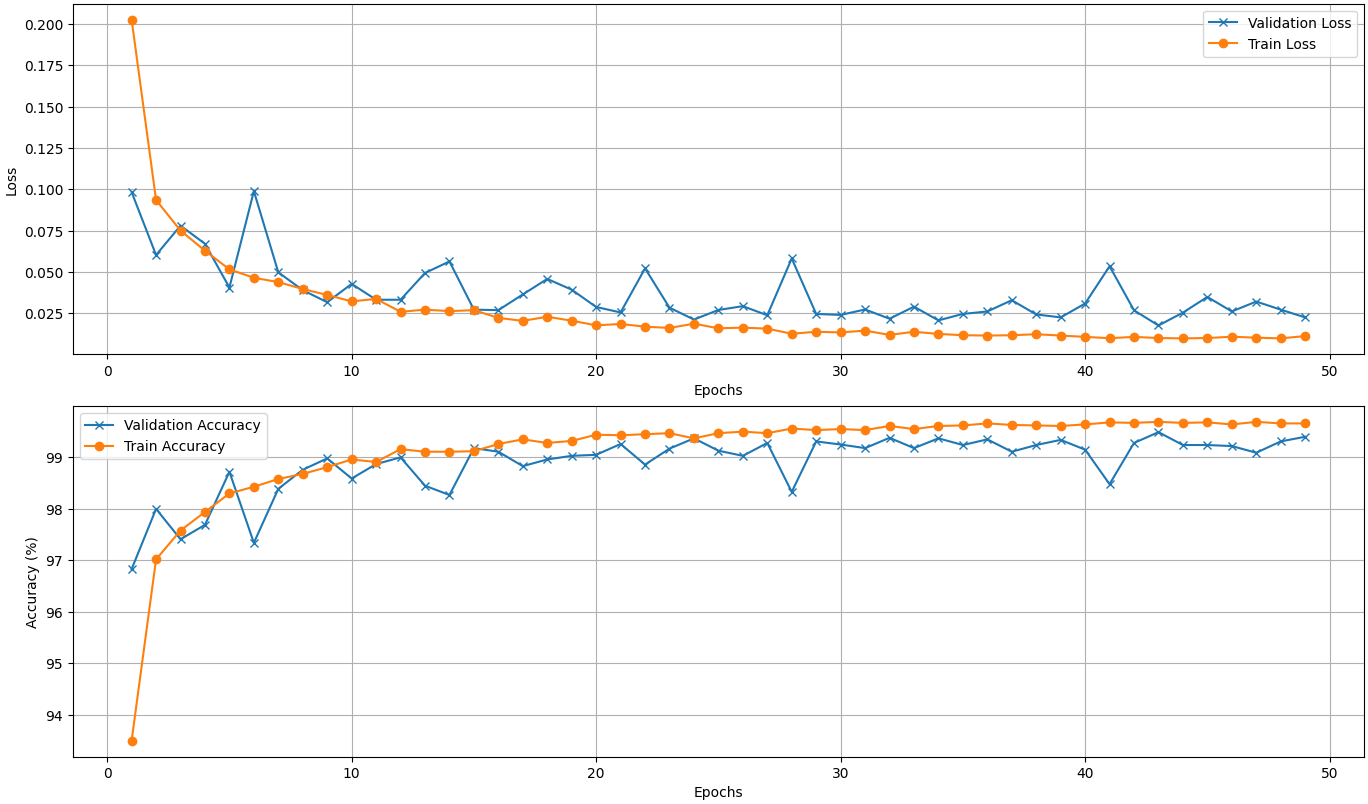
\includegraphics[width=.9\textwidth]{figures/xception_PathMNIST_result.png}
    \caption{}\label{fig:xception_PathMNIST}
\end{figure}